% Provenance (never printed): cycle 3 "La planete Terre" (natural phenomena
% and the risks they bring: storms, floods, droughts, earthquakes, eruptions;
% warnings and the right behaviour); see sources/book1/PROVENANCE.md.
% Book 1, grade 5, chapter 3.
\chapter{Los peligros naturales}\label{ch:g5:natural-hazards}

Es viernes por la tarde. En la radio, la música se interrumpe y una voz
tranquila lee un aviso: esta noche llegará a la \omterm{def:g1:landscapes-around-us:water}{costa} una fuerte \omterm{def:g5:natural-hazards:storm}{tormenta},
con vientos muy fuertes y \omterm{def:g4:clouds-rain-snow:precipitation}{lluvias} intensas. Se pide a la gente que no salga
de casa a partir de las nueve y que ate o meta dentro todo lo que el viento
pueda llevarse.

La familia de Lena se pone manos a la obra. Su padre mete en el cobertizo
las sillas y la mesa del jardín. Su madre comprueba que las linternas
funcionan y deja pilas de repuesto en la mesa de la cocina. Lena llena de
agua dos botellas grandes. A las nueve están todos dentro, y el viento ya
aúlla.

\begin{omfigure}
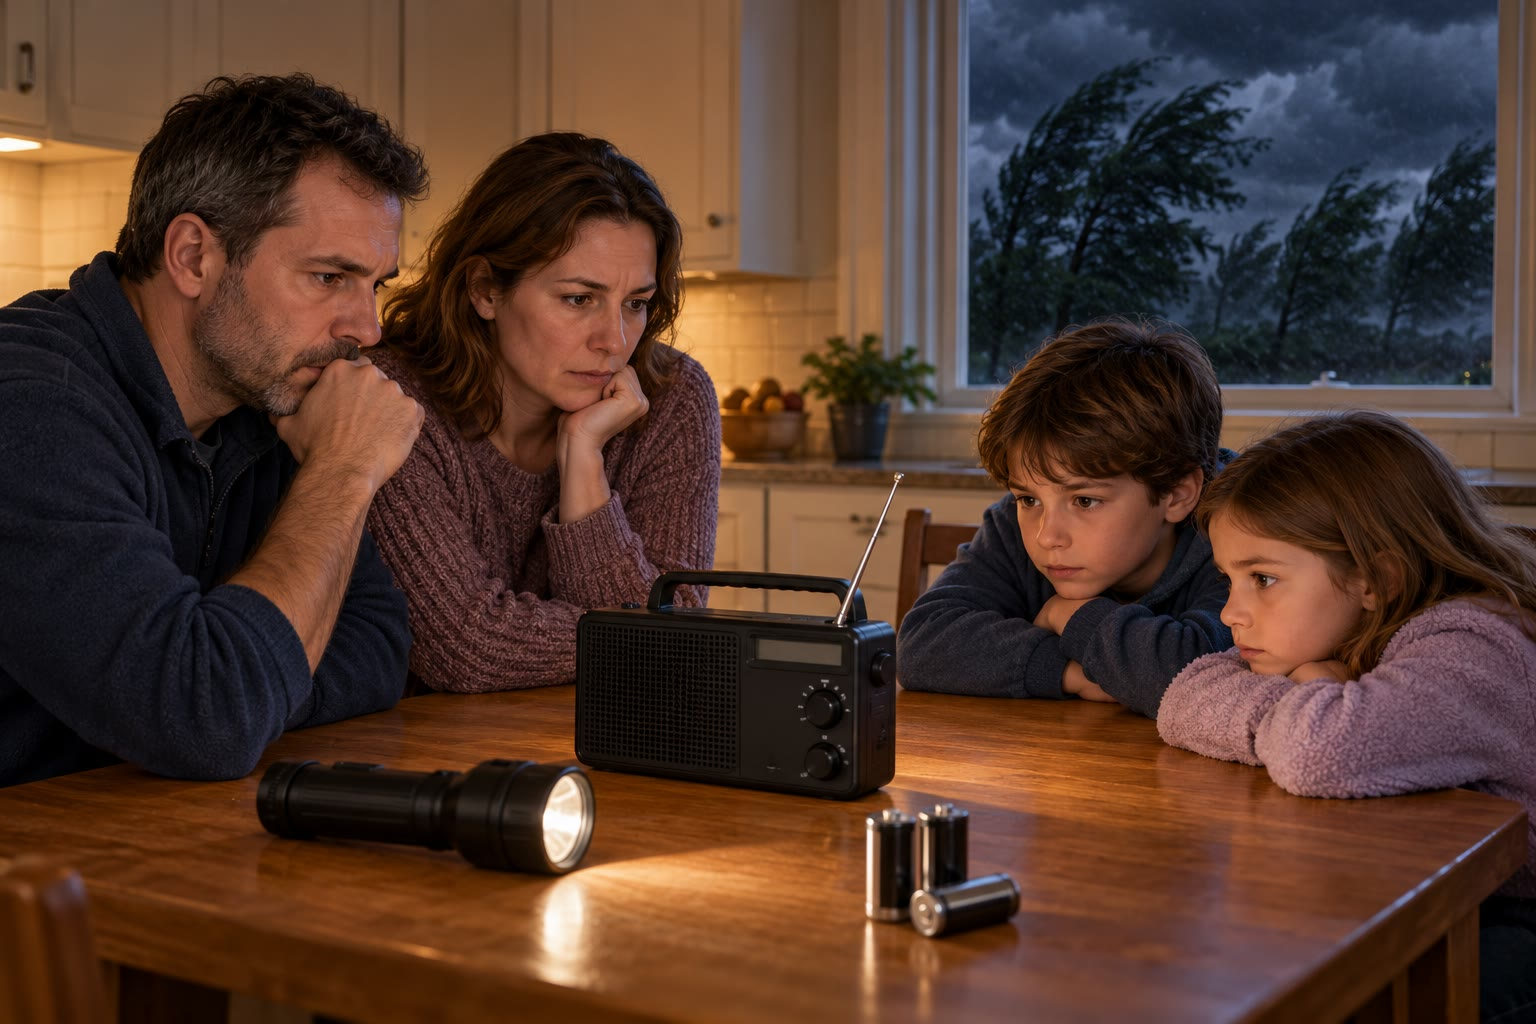
\includegraphics[width=0.5\linewidth]{images/book1/ai/g5-radio-warning.jpg}

{\small Una familia escucha un aviso de \omterm{def:g5:natural-hazards:storm}{tormenta} en la radio, con las
linternas y las pilas de repuesto preparadas.}
\end{omfigure}

\begin{recall}
Un \omterm{def:g4:volcanoes-earthquakes-first-look:volcano}{volcán} puede entrar en \omterm{def:g4:volcanoes-earthquakes-first-look:eruption}{erupción} y expulsar \omterm{def:g4:volcanoes-earthquakes-first-look:eruption}{lava}, ceniza y gases; un
\omterm{def:g4:volcanoes-earthquakes-first-look:earthquake}{terremoto} es una sacudida brusca del suelo; durante un \omterm{def:g4:volcanoes-earthquakes-first-look:earthquake}{terremoto}, nos
agachamos, nos cubrimos y nos agarramos
(\cref{ch:g4:volcanoes-earthquakes-first-look}). Un \omterm{def:g1:landscapes-around-us:water}{río} que recibe más agua
de la que cabe en su cauce inunda su \omterm{def:g5:water-shapes-the-land:flood}{llanura de inundación}
(\cref{ch:g5:water-shapes-the-land}). Cada lugar tiene su propio \omterm{def:g5:weather-and-climate:climate}{clima}, y
las zonas cálida, templadas y frías dan la vuelta al \omterm{def:g3:continents-and-oceans:globe}{globo}
(\cref{ch:g5:weather-and-climate}).
\end{recall}

\section{Qué es un peligro natural}

La naturaleza no siempre está en calma. El viento puede soplar con fuerza
suficiente para romper árboles, los \omterm{def:g1:landscapes-around-us:water}{ríos} pueden desbordarse, el suelo puede
temblar. Estos fenómenos forman parte del funcionamiento de la Tierra: ya
ocurrían mucho antes de que hubiera personas, y seguirán ocurriendo.

\begin{definition}[Peligro natural]\label{def:g5:natural-hazards:hazard}
Un \emph{peligro natural}\index{peligro natural} es un fenómeno natural que
puede hacer daño a las personas o destruir lo que han construido: una
\omterm{def:g5:natural-hazards:storm}{tormenta}, una \omterm{def:g5:water-shapes-the-land:flood}{inundación}, una \omterm{def:g5:natural-hazards:drought}{sequía}, un \omterm{def:g4:volcanoes-earthquakes-first-look:earthquake}{terremoto}, una \omterm{def:g4:volcanoes-earthquakes-first-look:eruption}{erupción} volcánica,
un \omterm{def:g5:natural-hazards:landslide}{deslizamiento de tierra}{\ldots}
\end{definition}

Podemos clasificar los \omterm{def:g5:natural-hazards:hazard}{peligros naturales} según su origen: el aire, el agua
o el suelo.

\begin{omfigure}
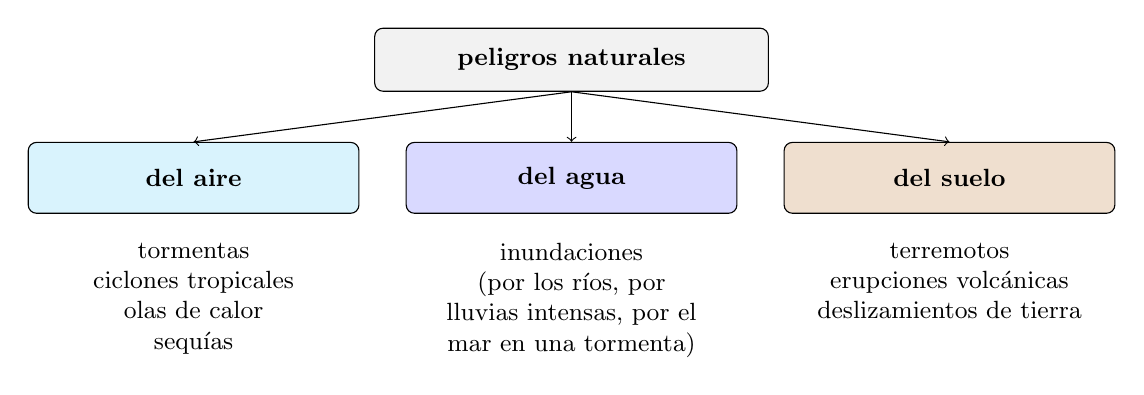
\begin{tikzpicture}[font=\small, box/.style={draw, rounded corners=3pt,
    minimum width=4.2cm, minimum height=0.9cm, align=center}]
  \node[box, fill=cyan!15, font=\small\bfseries] (A) at (0,0) {del aire};
  \node[box, fill=blue!15, font=\small\bfseries] (W) at (4.8,0) {del agua};
  \node[box, fill=brown!25, font=\small\bfseries] (G) at (9.6,0) {del suelo};
  \node[align=center, anchor=north] at (0,-0.7) {tormentas\\ciclones tropicales\\olas de calor\\sequías};
  \node[align=center, anchor=north] at (4.8,-0.7) {inundaciones\\(por los ríos, por\\lluvias intensas, por el\\mar en una tormenta)};
  \node[align=center, anchor=north] at (9.6,-0.7) {terremotos\\erupciones volcánicas\\deslizamientos de tierra};
  \node[draw, rounded corners=3pt, fill=gray!10, font=\small\bfseries,
    minimum width=5cm, minimum height=0.8cm] (N) at (4.8,1.5) {peligros naturales};
  \draw[->] (N.south) -- (A.north);
  \draw[->] (N.south) -- (W.north);
  \draw[->] (N.south) -- (G.north);
\end{tikzpicture}

{\small Los \omterm{def:g5:natural-hazards:hazard}{peligros naturales}, clasificados según su origen.}
\end{omfigure}

\section{Peligros que vienen del aire}

\begin{definition}[Tormenta]\label{def:g5:natural-hazards:storm}
Una \emph{tormenta}\index{tormenta} es un periodo de viento muy fuerte,
normalmente con \omterm{def:g4:clouds-rain-snow:precipitation}{lluvia} o \omterm{def:g4:clouds-rain-snow:precipitation}{nieve} intensas, y a veces con truenos y relámpagos.
\end{definition}

Una \omterm{def:g5:natural-hazards:storm}{tormenta} fuerte rompe ramas, derriba árboles, arranca tejas de los
tejados y puede lanzar sillas de jardín contra las ventanas. En la \omterm{def:g1:landscapes-around-us:water}{costa},
su viento empuja el \omterm{def:g2:water-on-earth:ocean}{mar} contra la orilla y lanza olas enormes por encima de
los diques.

Las \omterm{def:g5:natural-hazards:storm}{tormentas} más potentes de la Tierra se forman sobre los \omterm{def:g2:water-on-earth:ocean}{mares}
tropicales cálidos. Son \omterm{def:g5:natural-hazards:storm}{tormentas} enormes que giran sobre sí mismas: desde
el espacio parecen una espiral gigante de \omterm{def:g4:clouds-rain-snow:cloud}{nubes}, con un agujero tranquilo y
despejado en el centro, el ojo. Alrededor del ojo soplan los vientos más
fuertes. El mismo tipo de \omterm{def:g5:natural-hazards:storm}{tormenta} tiene nombres distintos en \omterm{def:g2:water-on-earth:ocean}{océanos}
distintos: se llama \emph{huracán} en el Atlántico Norte y en el Pacífico
oriental, \emph{tifón} en el Pacífico noroccidental y \emph{ciclón
tropical} en el Pacífico Sur y en el \omterm{def:g2:water-on-earth:ocean}{océano} Índico.
% ledger: noaa:cyclone-names

\begin{omfigure}
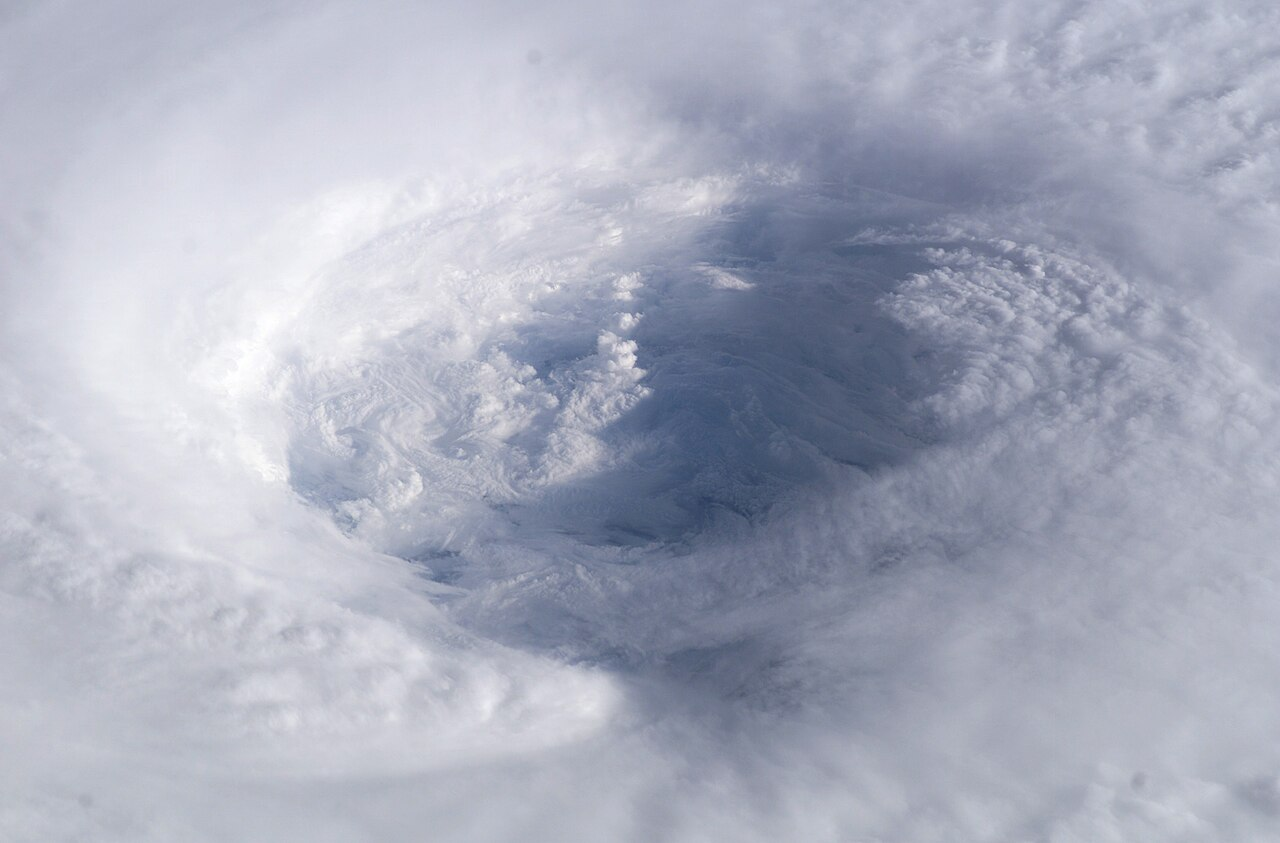
\includegraphics[width=0.5\linewidth]{images/book1/g5-hurricane-isabel-iss.jpg}

{\small Mirando hacia abajo, al ojo del huracán Isabel, sobre el \omterm{def:g2:water-on-earth:ocean}{océano}
Atlántico, en septiembre de 2003, desde la Estación Espacial
Internacional: una pared de \omterm{def:g4:clouds-rain-snow:cloud}{nubes} alrededor de un centro más tranquilo.
Fotografía: NASA (dominio público).}
% ledger: nasa:isabel-iss
\end{omfigure}

Algunos peligros que vienen del aire son lentos y silenciosos. Una \emph{ola
de calor} es un periodo de varios días y noches mucho más calurosos de lo
habitual. Es peligrosa sobre todo para las personas muy mayores, los bebés
y los enfermos.

\begin{definition}[Sequía]\label{def:g5:natural-hazards:drought}
Una \emph{sequía}\index{sequia@sequía} es un periodo largo, de meses o
incluso de años, con mucha menos \omterm{def:g4:clouds-rain-snow:precipitation}{lluvia} de la habitual en ese lugar. El
suelo se seca, los \omterm{def:g1:landscapes-around-us:water}{ríos} y los \omterm{def:g1:landscapes-around-us:water}{lagos} menguan, y los cultivos se marchitan y
mueren.
\end{definition}

Una \omterm{def:g5:natural-hazards:drought}{sequía} llega poco a poco: nadie puede decir qué día empieza. Pero una
\omterm{def:g5:natural-hazards:drought}{sequía} larga puede dejar a los agricultores sin cosecha y a las ciudades
sin agua suficiente.

\begin{omfigure}
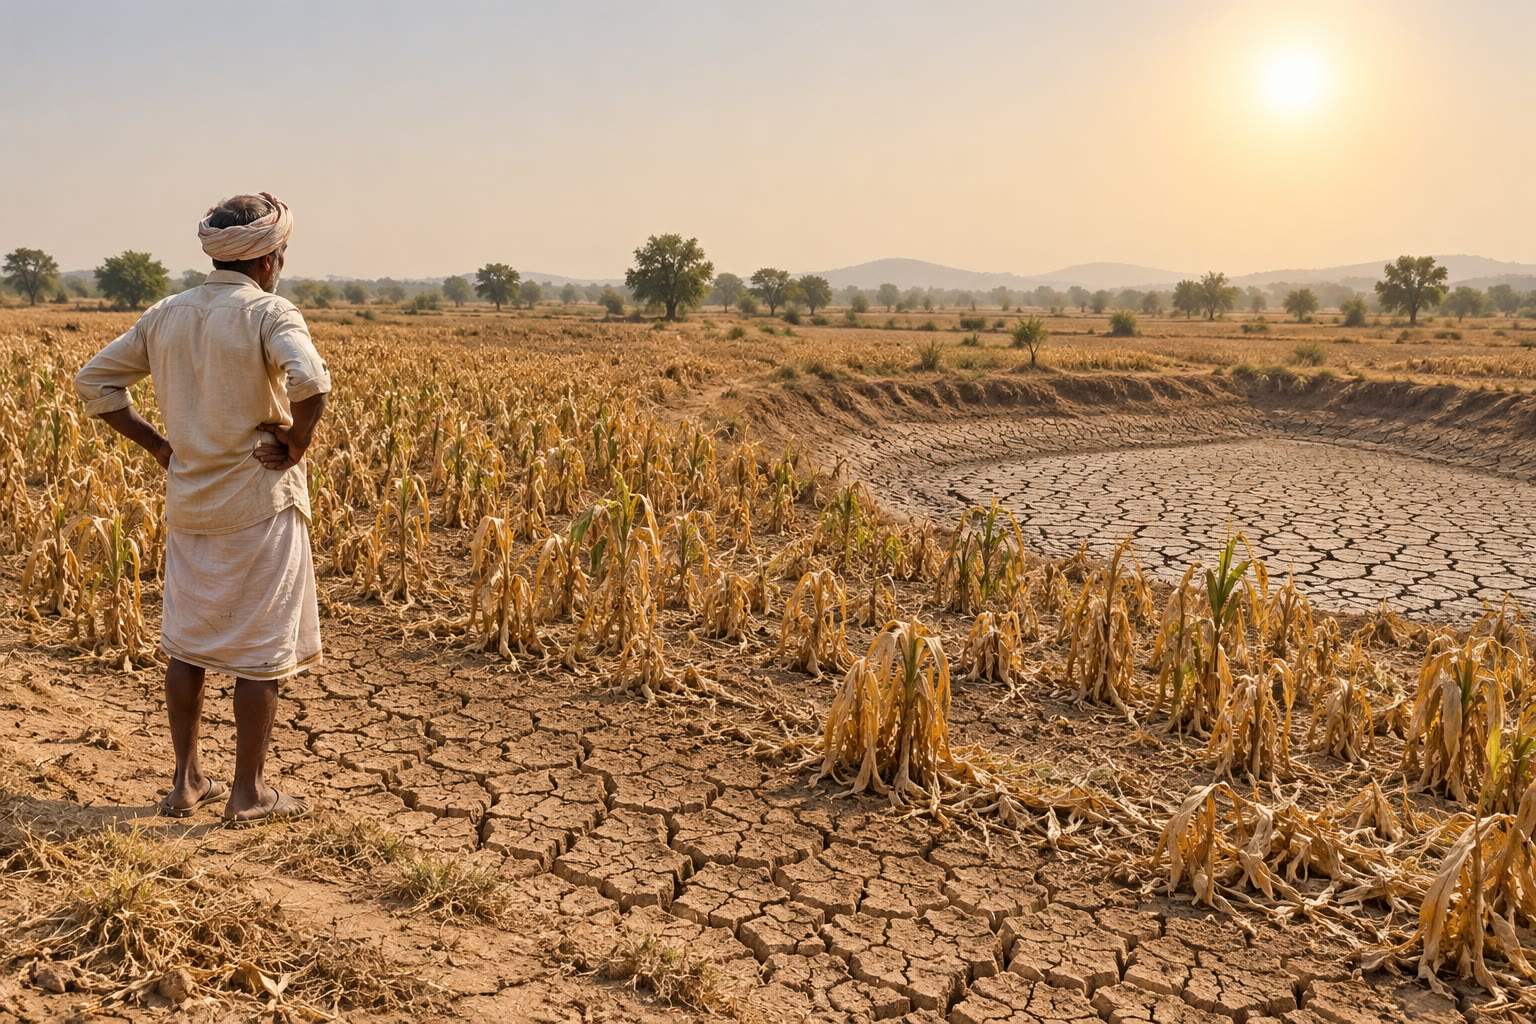
\includegraphics[width=0.42\linewidth]{images/book1/ai/g5-drought-field.jpg}

{\small Un campo durante una \omterm{def:g5:natural-hazards:drought}{sequía} larga: la tierra está agrietada, los
cultivos están amarillos y la charca se ha secado.}
\end{omfigure}

\section{Peligros que vienen del agua}

Ya conoces las \omterm{def:g5:water-shapes-the-land:flood}{inundaciones} de los \omterm{def:g1:landscapes-around-us:water}{ríos} (\cref{ch:g5:water-shapes-the-land}).
Después de días de \omterm{def:g4:clouds-rain-snow:precipitation}{lluvia}, o cuando la \omterm{def:g4:clouds-rain-snow:precipitation}{nieve} se funde deprisa, un \omterm{def:g1:landscapes-around-us:water}{río} sube
por encima de sus orillas y cubre su \omterm{def:g5:water-shapes-the-land:flood}{llanura de inundación}. Algunas
\omterm{def:g5:water-shapes-the-land:flood}{inundaciones} llegan muy deprisa: un aguacero violento sobre un \omterm{def:g1:landscapes-around-us:landform}{valle}
empinado puede convertir un arroyo tranquilo en un torrente rugiente en
menos de una hora. Otras vienen del \omterm{def:g2:water-on-earth:ocean}{mar}, cuando una \omterm{def:g5:natural-hazards:storm}{tormenta} empuja el agua
sobre una \omterm{def:g1:landscapes-around-us:water}{costa} baja.

\section{Peligros que vienen del suelo}

Ya conoces los \omterm{def:g4:volcanoes-earthquakes-first-look:earthquake}{terremotos} y las \omterm{def:g4:volcanoes-earthquakes-first-look:eruption}{erupciones} volcánicas
(\cref{ch:g4:volcanoes-earthquakes-first-look}). Hay un tercer peligro que
viene del suelo, y a menudo lo desencadena el agua.

\begin{definition}[Deslizamiento de tierra]\label{def:g5:natural-hazards:landslide}
Un \emph{deslizamiento de tierra}\index{deslizamiento de tierra} es una
masa de \omterm{def:g3:stones-pebbles-sand:rock}{roca}, tierra o \omterm{def:g3:stones-pebbles-sand:sand}{barro} que de repente se desliza o cae por una
pendiente.
\end{definition}

Una pendiente empinada empapada por \omterm{def:g4:clouds-rain-snow:precipitation}{lluvias} largas se vuelve pesada y
resbaladiza, y puede soltarse de golpe. Un \omterm{def:g4:volcanoes-earthquakes-first-look:earthquake}{terremoto} también puede sacudir
una pendiente hasta desprenderla. Un \omterm{def:g5:natural-hazards:landslide}{deslizamiento de tierra} puede sepultar
una carretera, cortar un \omterm{def:g1:landscapes-around-us:water}{río} o llevarse casas.

\begin{omfigure}
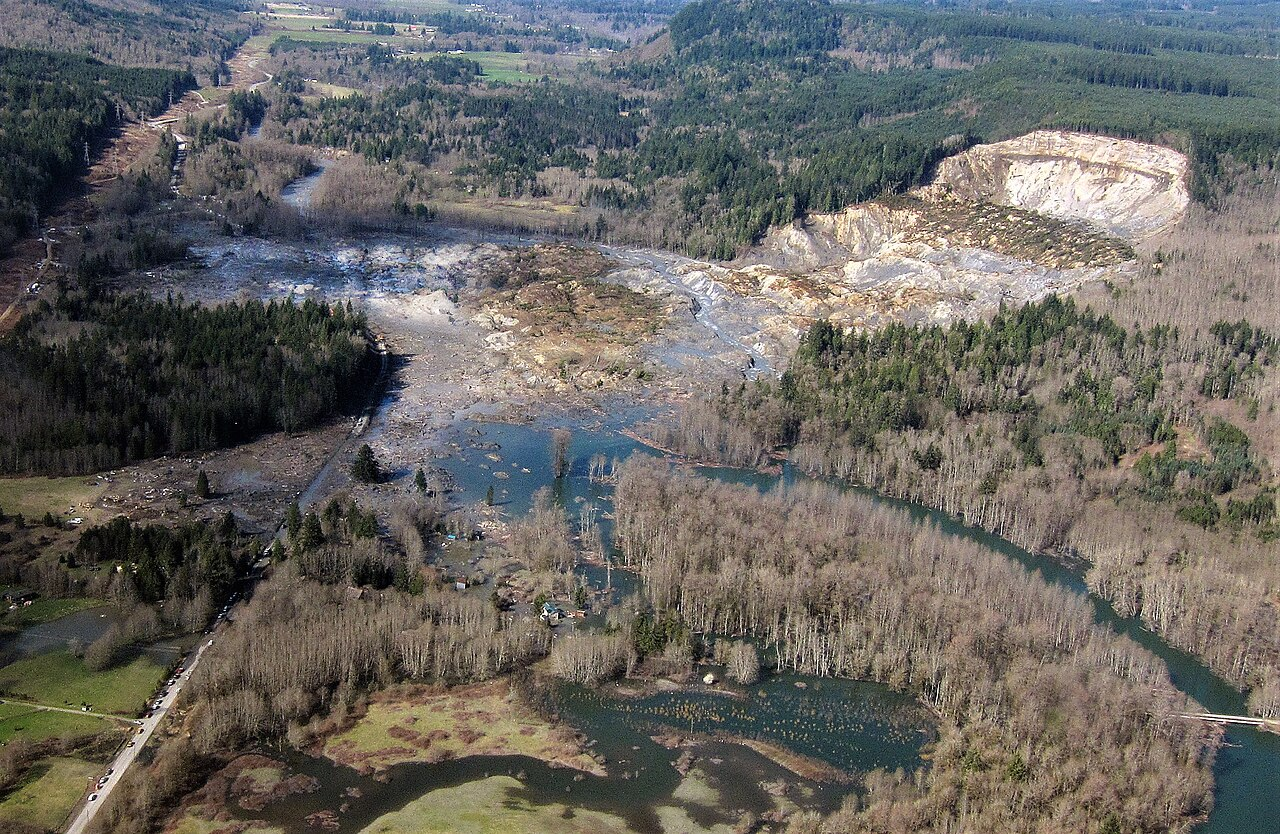
\includegraphics[width=0.6\linewidth]{images/book1/g5-landslide-washington.jpg}

{\small Un gran \omterm{def:g5:natural-hazards:landslide}{deslizamiento de tierra} en el estado de Washington, en los
Estados Unidos, en 2014, visto desde un avión. La ladera de la derecha se ha
derrumbado; su \omterm{def:g3:stones-pebbles-sand:sand}{barro} se ha extendido por todo el \omterm{def:g1:landscapes-around-us:landform}{valle}, ha cubierto una
carretera y ha cortado el \omterm{def:g1:landscapes-around-us:water}{río}, que ha inundado el bosque de \omterm{def:g1:landscapes-around-us:water}{río} arriba.
Fotografía: Mark Reid, U.S. Geological Survey (dominio
público).}\label{fig:g5:natural-hazards:landslide}
% ledger: usgs:oso-aerial
\end{omfigure}

\section{Del peligro a la catástrofe}

Una \omterm{def:g5:natural-hazards:storm}{tormenta} en \omterm{def:g2:water-on-earth:ocean}{mar} abierto, un \omterm{def:g4:volcanoes-earthquakes-first-look:earthquake}{terremoto} en un \omterm{def:g5:weather-and-climate:desert}{desierto} vacío, una
\omterm{def:g5:water-shapes-the-land:flood}{inundación} en un \omterm{def:g1:landscapes-around-us:landform}{valle} donde no vive nadie: son \omterm{def:g5:natural-hazards:hazard}{peligros naturales}, pero no
hacen daño a nadie. Los mismos fenómenos se vuelven peligrosos cuando
golpean donde vive la gente.

\begin{definition}[Catástrofe natural]\label{def:g5:natural-hazards:disaster}
Hay una \emph{catástrofe natural}\index{catastrofe natural@catástrofe natural}
cuando un \omterm{def:g5:natural-hazards:hazard}{peligro natural} golpea un lugar donde vive gente y causa un gran
daño: hay heridos o muertos, se destruyen viviendas, y se cortan las
carreteras, el agua y la electricidad.
\end{definition}

\begin{omfigure}
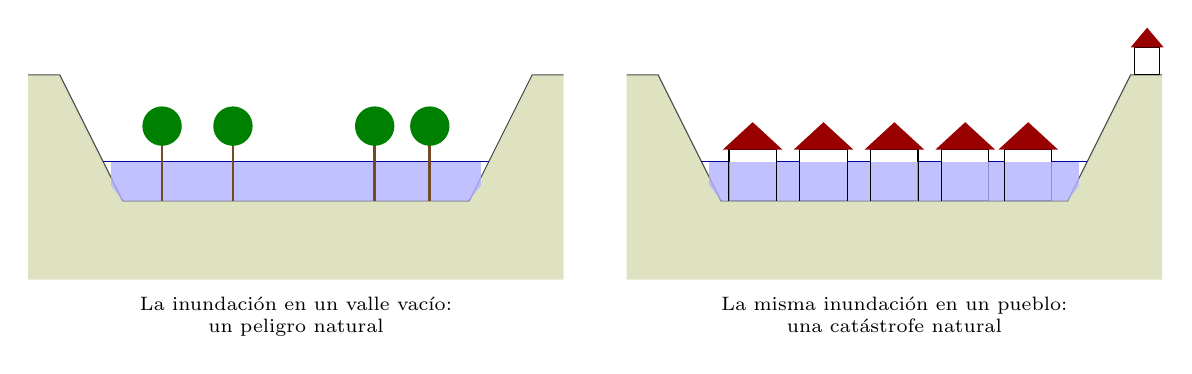
\begin{tikzpicture}[x=1cm, y=1cm, font=\scriptsize]
  \foreach \dx/\title in {0/{La inundación en un valle vacío:\\un peligro natural},
                          7.6/{La misma inundación en un pueblo:\\una catástrofe natural}} {
    \begin{scope}[xshift=\dx cm]
      % valley sides
      \fill[green!25!brown!30] (0,0) -- (0,2.6) -- (0.4,2.6) -- (1.2,1.0) -- (5.6,1.0)
        -- (6.4,2.6) -- (6.8,2.6) -- (6.8,0) -- cycle;
      \draw[gray!60!black] (0,2.6) -- (0.4,2.6) -- (1.2,1.0) -- (5.6,1.0) -- (6.4,2.6) -- (6.8,2.6);
      % flood water over the whole valley floor
      \fill[blue!30, opacity=0.8] (1.05,1.2) -- (5.75,1.2) -- (5.6,1.0) -- (1.2,1.0) -- cycle;
      \fill[blue!30, opacity=0.8] (1.05,1.2) rectangle (5.75,1.5);
      \draw[blue!60!black] (0.95,1.5) -- (5.85,1.5);
      \node[align=center, anchor=north] at (3.4,-0.1) {\title};
    \end{scope}
  }
  % trees in the empty valley
  \foreach \x in {1.7,2.6,4.4,5.1} {
    \draw[brown!60!black, line width=1pt] (\x,1.0) -- (\x,1.75);
    \fill[green!50!black] (\x,1.95) circle (0.25);
  }
  % houses in the village valley
  \begin{scope}[xshift=7.6cm]
    \foreach \x in {1.6,2.5,3.4,4.3,5.1} {
      \fill[white, draw=black] (\x-0.3,1.0) rectangle (\x+0.3,1.65);
      \fill[red!60!black] (\x-0.38,1.65) -- (\x,2.0) -- (\x+0.38,1.65) -- cycle;
      \fill[blue!30, opacity=0.8] (\x-0.3,1.0) rectangle (\x+0.3,1.5);
    }
    % one house on the high ground, dry
    \fill[white, draw=black] (6.45,2.6) rectangle (6.77,2.95);
    \fill[red!60!black] (6.40,2.95) -- (6.61,3.2) -- (6.82,2.95) -- cycle;
  \end{scope}
\end{tikzpicture}

{\small La misma \omterm{def:g5:water-shapes-the-land:flood}{inundación}, dos veces. En el \omterm{def:g1:landscapes-around-us:landform}{valle} vacío no hace daño a
nadie; donde se ha construido un pueblo en la \omterm{def:g5:water-shapes-the-land:flood}{llanura de inundación}, llena
de agua las casas. La casa del terreno alto se queda seca.}
\end{omfigure}

No podemos detener una \omterm{def:g5:natural-hazards:storm}{tormenta} ni un \omterm{def:g4:volcanoes-earthquakes-first-look:earthquake}{terremoto}. Pero podemos hacer mucho
para que un peligro no se convierta en una catástrofe: construir lejos de
las \omterm{def:g5:water-shapes-the-land:flood}{llanuras de inundación} y del pie de las pendientes inestables, hacer
edificios sólidos, vigilar el \omterm{def:g1:watching-the-weather:weather}{tiempo} y el suelo, avisar a la gente a tiempo
y enseñar a todos lo que hay que hacer.

\subsection*{Los avisos}

Los servicios meteorológicos vigilan el cielo día y noche. Cuando se acerca
una \omterm{def:g5:natural-hazards:storm}{tormenta}, una ola de calor o una \omterm{def:g5:water-shapes-the-land:flood}{inundación}, emiten avisos por la radio,
la televisión, el teléfono e internet. Muchos países usan colores, del más
tranquilo al más grave.

\begin{omfigure}
\begin{tikzpicture}[font=\small, wstep/.style={draw=black!60, minimum width=2.6cm,
    minimum height=0.8cm, font=\small\bfseries, rounded corners=2pt}]
  \node[wstep, fill=green!45] (g) at (0,0) {verde};
  \node[wstep, fill=yellow!60] (y) at (0.6,0.95) {amarillo};
  \node[wstep, fill=orange!70] (o) at (1.2,1.9) {naranja};
  \node[wstep, fill=red!65, text=white] (r) at (1.8,2.85) {rojo};
  \node[anchor=west] at ($(g.east)+(0.3,0)$) {ningún peligro especial};
  \node[anchor=west] at ($(y.east)+(0.3,0)$) {ten cuidado, mantente informado};
  \node[anchor=west] at ($(o.east)+(0.3,0)$) {prepárate: el peligro es probable};
  \node[anchor=west] at ($(r.east)+(0.3,0)$) {gran peligro: actúa ya, sigue las instrucciones};
\end{tikzpicture}

{\small Una escala de colores de aviso. El significado exacto cambia de un
país a otro: escucha siempre las instrucciones que acompañan al aviso.}
\end{omfigure}

\begin{safety}
\textbf{Durante una \omterm{def:g5:natural-hazards:storm}{tormenta}.} Quédate dentro, lejos de las ventanas. No
salgas a mirar, y mantente lejos de los árboles, que pueden caerse, y de los
cables eléctricos caídos.

\textbf{Durante una \omterm{def:g5:water-shapes-the-land:flood}{inundación}.} Sube a un terreno más alto o a un piso
superior. No atravieses nunca el agua de una \omterm{def:g5:water-shapes-the-land:flood}{inundación} a pie, en bici ni en
coche: basta un poco de agua rápida para tirarte al suelo o llevarse un
coche.

\textbf{Durante una ola de calor.} Bebe agua a menudo, quédate a la sombra o
en una habitación fresca durante las horas de más calor, y pregunta cómo
están los vecinos mayores.

\textbf{Durante un \omterm{def:g4:volcanoes-earthquakes-first-look:earthquake}{terremoto}.} Agáchate, cúbrete, agárrate
(\cref{ch:g4:volcanoes-earthquakes-first-look}).

\textbf{Siempre.} Escucha los avisos y haz enseguida lo que digan los
responsables.
\end{safety}

\section{Ejercicios}

\begin{exercise}[$\star$]\label{exo:g5:natural-hazards:1}
¿Solo un \omterm{def:g5:natural-hazards:hazard}{peligro natural}, o una \omterm{def:g5:natural-hazards:disaster}{catástrofe natural}?
\begin{enumerate}
  \item[(a)] Un \omterm{def:g4:volcanoes-earthquakes-first-look:earthquake}{terremoto} sacude un \omterm{def:g5:weather-and-climate:desert}{desierto} vacío.
  \item[(b)] Una \omterm{def:g5:natural-hazards:storm}{tormenta} arranca los tejados de muchas casas de una ciudad.
  \item[(c)] Un \omterm{def:g5:natural-hazards:landslide}{deslizamiento de tierra} cae en un \omterm{def:g1:landscapes-around-us:landform}{valle} de \omterm{def:g1:landscapes-around-us:landform}{montaña} donde no
        vive nadie.
  \item[(d)] Un \omterm{def:g1:landscapes-around-us:water}{río} inunda un pueblo y llena sus casas de agua.
\end{enumerate}
\end{exercise}

\begin{exercise}[$\star$]\label{exo:g5:natural-hazards:2}
Clasifica estos peligros en tres familias (del aire, del agua, del suelo):
un \omterm{def:g5:natural-hazards:landslide}{deslizamiento de tierra}; una ola de calor; una \omterm{def:g5:water-shapes-the-land:flood}{inundación}; una \omterm{def:g4:volcanoes-earthquakes-first-look:eruption}{erupción}
volcánica; una \omterm{def:g5:natural-hazards:storm}{tormenta}; una \omterm{def:g5:natural-hazards:drought}{sequía}; un \omterm{def:g4:volcanoes-earthquakes-first-look:earthquake}{terremoto}.
\end{exercise}

\begin{exercise}[$\star$]\label{exo:g5:natural-hazards:3}
¿Qué es una \omterm{def:g5:natural-hazards:drought}{sequía}? Di dos maneras en que una \omterm{def:g5:natural-hazards:drought}{sequía} larga perjudica a las personas.
\end{exercise}

\begin{exercise}[$\star$]\label{exo:g5:natural-hazards:4}
La radio anuncia un aviso rojo por \omterm{def:g5:natural-hazards:storm}{tormenta} para esta noche. Di tres cosas
que debería hacer tu familia.
\end{exercise}

\begin{exercise}[$\star$]\label{exo:g5:natural-hazards:5}
Sobre un \omterm{def:g2:water-on-earth:ocean}{mar} tropical cálido se forma una gran \omterm{def:g5:natural-hazards:storm}{tormenta} giratoria con un
ojo. ¿Cómo se llama si llega (a) a la \omterm{def:g1:landscapes-around-us:water}{costa} de Florida, en el Atlántico
Norte; (b) a Japón, en el Pacífico noroccidental; (c) a la \omterm{def:g1:landscapes-around-us:water}{costa} de la
India, en el \omterm{def:g2:water-on-earth:ocean}{océano} Índico?
\end{exercise}

\begin{exercise}[$\star$]\label{exo:g5:natural-hazards:6}
Ordena los cuatro colores de aviso, del más tranquilo al más grave. ¿Qué
debes hacer en el nivel más grave?
\end{exercise}

\begin{exercise}[$\star\star$]\label{exo:g5:natural-hazards:7}
Mira la fotografía del \omterm{def:g5:natural-hazards:landslide}{deslizamiento de tierra} de la
página~\pageref{fig:g5:natural-hazards:landslide}. Describe lo que el
deslizamiento le hizo al \omterm{def:g1:landscapes-around-us:landform}{valle}: a la ladera, a la carretera y al \omterm{def:g1:landscapes-around-us:water}{río}. ¿Por
qué la tierra de \omterm{def:g1:landscapes-around-us:water}{río} arriba está ahora bajo el agua?
\end{exercise}

\begin{exercise}[$\star\star$]\label{exo:g5:natural-hazards:8}
Tom dice: ``Las \omterm{def:g5:water-shapes-the-land:flood}{inundaciones} son naturales, así que no se puede hacer nada
contra ellas''. Lena dice: ``No podemos impedir que un \omterm{def:g1:landscapes-around-us:water}{río} se desborde, pero
sí podemos impedir que una \omterm{def:g5:water-shapes-the-land:flood}{inundación} se convierta en una catástrofe''.
¿Quién tiene razón? Explícalo con dos ejemplos.
\end{exercise}

\begin{exercise}[$\star\star$]\label{exo:g5:natural-hazards:9}
En una región agrícola imaginaria caen normalmente unos 60 milímetros de
\omterm{def:g4:clouds-rain-snow:precipitation}{lluvia} cada mes. Durante una \omterm{def:g5:natural-hazards:drought}{sequía}, solo cayó una cuarta parte de la \omterm{def:g4:clouds-rain-snow:precipitation}{lluvia}
habitual en cada uno de cuatro meses.
\begin{enumerate}
  \item[(a)] ¿Cuánta \omterm{def:g4:clouds-rain-snow:precipitation}{lluvia} cae normalmente en cuatro meses?
  \item[(b)] ¿Cuánta cayó durante la \omterm{def:g5:natural-hazards:drought}{sequía}, en los cuatro meses?
  \item[(c)] ¿Cuánta \omterm{def:g4:clouds-rain-snow:precipitation}{lluvia} faltó?
\end{enumerate}
\end{exercise}

\begin{exercise}[$\star\star$]\label{exo:g5:natural-hazards:10}
Una ciudad imaginaria tiene 1\,200 viviendas. Una cuarta parte de ellas
están en la \omterm{def:g5:water-shapes-the-land:flood}{llanura de inundación} de su \omterm{def:g1:landscapes-around-us:water}{río}.
\begin{enumerate}
  \item[(a)] ¿Cuántas viviendas están en la \omterm{def:g5:water-shapes-the-land:flood}{llanura de inundación}?
  \item[(b)] La ciudad ayuda a los propietarios de un tercio de esas
        viviendas a trasladarse a un terreno más alto. ¿Cuántas viviendas
        siguen en la \omterm{def:g5:water-shapes-the-land:flood}{llanura de inundación}?
\end{enumerate}
\end{exercise}

\begin{exercise}[$\star\star\star$]\label{exo:g5:natural-hazards:11}
Dos pueblos, muy alejados entre sí, sufren la misma noche \omterm{def:g5:natural-hazards:storm}{tormentas} de la
misma fuerza. En el primero no hay heridos y los daños son pequeños. En el
segundo se destruyen muchas casas. Da al menos tres razones distintas que
podrían explicar la diferencia.
\end{exercise}
